\section{Past Work}
\label{sec:related}

Our works builds upon several areas of research, in particular the graphical representation of news articles, the identification and tracking of topics, time-based story and event evolution, multi document summarization, and information visualisation.

\paragraph*{Graph representation of Articles} Choudhary et al.\cite{choudhary@ecir2008} proposed (which was at that time) a novel method of organizing a news corpus into a directed graph, by mining and tracking the \emph{transformations} that the entities in the corpus undergo. These transformations, defined for one or more entities, can be one of the following:
\squishlist
  \item \textbf{Birth:} An entity appearing for the first time
  \item \textbf{Cease:} An entity appearing for the last time
  \item \textbf{Merge:} Two entities co-occurring for the first time
  \item \textbf{Split:} Two entities co-occurring for the last time
  \item \textbf{Continue:} An entity remaining popular in a period
\squishend
Their idea can be summarized as follows: 1) Mine transformations in the article set 2) Find a weighted-edge covering of all transformations.
For a more detailed description, we refer the reader to the paper. The work does not discuss how such a news graph may be mined to extract
useful information, rather proposes this graph as a means of visualizing the news. However, such graphs easily blow up as the complexity
of the news story increases. 

Figure~\ref{fig:sample-news-graph} shows an example graph that gets created using this technique for a set of 4
articles covering a crime story. Nodes $A$ and $B$ talk about the incident being reported, reactions from various sections of the society and
the progress of investigation. Then, there is a fork in the story, with node $C$ talking about the fate of the investigating officer Damayanti Sen, 
and node $D$ talks covers the judicial probe of the incident. The nodes $C$ and $D$ cover different different aspects of the same story.
\begin{figure}
\caption{A news graph of a crime incident from Bengal}
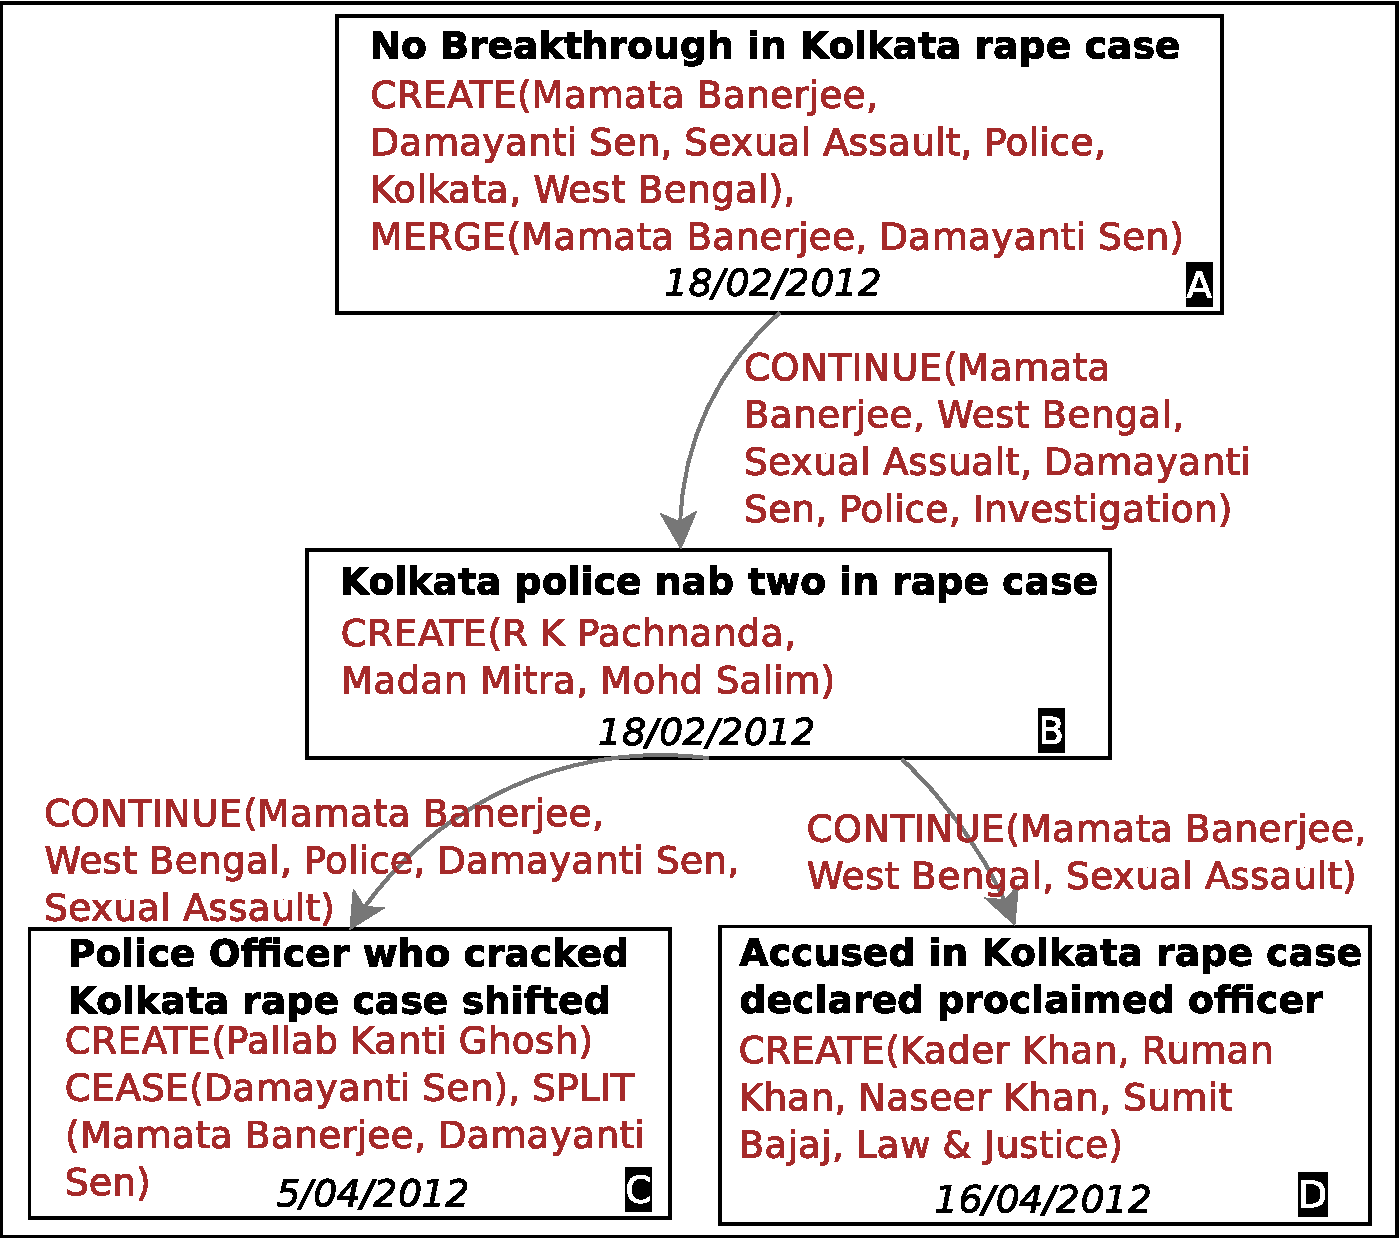
\includegraphics[scale=0.36]{figures/graph-1.pdf}
\label{fig:sample-news-graph}
\end{figure}
\paragraph*{Topic Detection and Tracking} Topic Detection \& Tracking (TDT) is a well studied problem \cite{springerlink:10.1023/B:INRT.0000011210.12953.86, springerlink:10.1007, Franz:2001:USC:383952.384013}. In TDT, a topic is defined as a collection of important words by considering documents to be bags-of-words. In ``Topic detection'', one determines clusters of articles that discuss the same topic, while in ``Topic tracking'', one detects stories that discuss a previously known topic \cite{Allan:2002:TDT:772260}. 

\paragraph*{Story Evolution}  Kim et al.\cite{Kim:2011:TCU:1964750.1964765} propose a method for detecting and tracking latent topics that appear within news articles, and visualize how the news corpus evolves from one topic set to another using topic similarity metrics. Suba\v{s}i\'{c} et al.\cite{subasic-ida:2013} %CONFIRM THIS IS THE RIGHT REFERENCE
 show how an event emerges, changes and disappears by dividing each event into several time stages and forming a network of co-occurence of terms based on frequency and time relevance. Nallapati et al.\cite
{Nallapati:2004:ETW:1031171.1031258, Mei:2005:DET:1081870.1081895} present a system to discover subtopics within a news topic and construct a graph showing their inter-dependencies. These systems are best-suited for simple linear news stories and may not work well for complex stories. In an extension to their previous work \cite{shahaf@kdd2010}, which finds the most coherent chain of articles that cover the story connecting 2 input articles, Shahaf et al.\cite{shahaf@www2012} construct a roadmap of chains of stories, which may have many branches of smaller stories. 

\paragraph*{Summarization} Barzilay et al.\cite{Barzilay:2002:ISS:1622810.1622812} talk about multidocument news summarization to generate a coherent and comprehensive summary from an input sequence of articles.

\paragraph*{Visualization} Vydiswaran et al.\cite{MEET:MEET14504801078} design a system to explore news by querying for topics, time range and locations. However, they process articles per user query. In addition, there is no notion of tracking news evolution on a timeline.

As far as we know, our work is the first attempt towards using a rich graph structure built out of the raw articles, that is amenable to repetitive querying without any significant cost of post-processing. Having such a structure, allows us to run efficient algorithms on the news article stream to mine and track the underlying news stories and to provide a personalised context to the story tailored to the user's query. Further, by visualizing these stories on a timeline, it helps the user follow the progression of the story through the different actors and topics.
